\renewcommand{\theequation}{\theenumi}
\begin{enumerate}[label=\thesection.\arabic*.,ref=\thesection.\theenumi]
\numberwithin{equation}{enumi}

%\renewcommand{\thefigure}{\theenumi.\arabic{figure}}
\begin{figure}[!ht]
\centering
\resizebox{\columnwidth}{!}{\input{./figs/circle.tex}}
\caption{Using Latex-Tikz}
\label{fig:circle_latex}	
\end{figure}
%
%
%\renewcommand{\thefigure}{\theenumi}
%
\item The following inputs were taken for constructing the figure:
\\
%
\begin{table}[ht!]
\centering
\input{./tables/inp.tex}
\caption{Input Table for construction}
\label{table:table1}	
\end{table}


\item The coordinates of  $\vec{A}$ and  $\vec{B}$ such that  $\vec{AB}$ is a diameter as in Fig. \ref{fig:circle_latex} are:
%\label{}
\\
%
%\solution From the given information, 
%$\triangle ABC$ are 
\begin{align}
\vec{A} &= \myvec{2\\0} ,
\label{eq:constr_a}
\\
 \vec{B} &= \myvec{-2\\0} 
\label{eq:constr_b}
\end{align}

\item 
Let $\vec{C}$ be a point on circle such that its coordinates are:
\begin{align}
\vec{C}= \myvec{1.414\\1.414}
\label{eq:constr_c}
\end{align}
Now $\vec{D}$ should be a point on the circle such that $\vec{CD}$ = 2 units (radius of the circle).
Let,
\begin{align}
\vec{D}= \myvec{x'\\y'}
\end{align}
So the coordinates of $\vec{D}$ will satisfy the following equations:
\begin{equation} \label{distance_formula}
(1.414-x')^{2} + (1.414-y')^{2} = 4  
\end{equation}
\begin{equation} \label{circle_eqn}
x'^{2} + y'^{2} = 4  
\end{equation}
Eqn. \ref{distance_formula} is the distance formula between two cordinates. Eqn. \ref{circle_eqn} is the equation of the circle with radius 2 units and centre at (0,0). \\
On solving these two euations, you get the value of \textit{x'} and \textit{y'}. So ,
\begin{align}
\vec{D}= \myvec{-0.518\\1.932}
\label{eq:constr_d}
\end{align}
\item The point $\vec{E}$ is obtained by the intersection of the extended lines of $\vec{AC}$ and $\vec{BD}$. \\
As the coordinates of points $\vec{A}$, $\vec{B}$, $\vec{C}$ and $\vec{D}$ are now known, you can find the line equation of $\vec{AC}$ and $\vec{BD}$.\\
By equating the line equations of $\vec{AC}$ and $\vec{BD}$, you get the intersection point i.e. point $\vec{E}$. \\
\begin{equation} \label{lineAC_eqn}
1.414x + 0.586y - 2.828 = 0
\end{equation}
\begin{equation} \label{lineBD_eqn}
1.932x - 1.482y + 3.864 = 0
\end{equation}
Eqn. \ref{lineAC_eqn} is the line equation of $\vec{AC}$ and Eqn. \ref{lineBD_eqn} is the line equation of $\vec{BD}$. \\ 
By solving these two equations, you get the coordinates of $\vec{E}$. 
\begin{align}
\vec{E}= \myvec{0.597\\3.385},
\label{eq:constr_e}
\end{align}
\item The derived values are listed in 
Table. \ref{table:table2} 
\begin{table}[ht!]
\centering
\input{./tables/derived.tex}
\caption{To construct $\triangle $ ABC}
\label{table:table2}
\end{table}
%
\item For solving the problem, join $\vec{OC}$, $\vec{OD}$ and $\vec{BC}$.
\item To get the python code for Fig \ref{fig:circle_python}, download it from
\begin{lstlisting}
codes/circle.py
\end{lstlisting}
\begin{figure}[!ht]
\centering
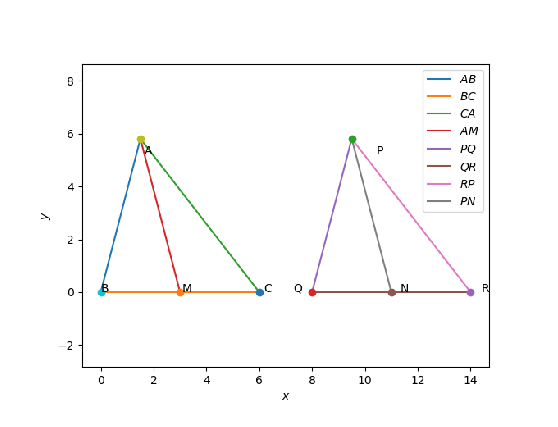
\includegraphics[width= \columnwidth]{Figure_1.eps}
\caption{Constructed using Python}
\label{fig:circle_python}
\end{figure}
%
and the equivalent latex-tikz code for Fig. \ref{fig:circle_latex} from
\begin{lstlisting}
figs/circle.tex
\end{lstlisting}
%
The above latex code can be compiled as a standalone document as
\begin{lstlisting}
figs/circle_fig.tex
\end{lstlisting}



\end{enumerate}